%!TEX program = xelatex
%!TEX options = --shell-escape

\documentclass[table, 14pt, aspectratio=169]{beamer}

\setbeamerfont{title}{series=\bfseries}
\setbeamerfont{frametitle}{series=\bfseries}
\usefonttheme[onlymath]{serif}

\definecolor{OxfordBlue}{RGB}{0, 33, 71}
\definecolor{OxfordGoldPale}{RGB}{243,222,116}
\setbeamercolor{title}{fg=OxfordBlue}
\setbeamercolor{frametitle}{fg=OxfordBlue}
\setbeamercolor{section in toc}{fg=black}
\setbeamercolor{description item}{fg=black}
\setbeamertemplate{description item}{\bfseries\insertdescriptionitem}
\setbeamercolor{local structure}{fg=OxfordBlue}
\setbeamertemplate{itemize item}{\color{OxfordBlue}$\blacktriangleright$}
\setbeamertemplate{itemize subitem}{\color{OxfordBlue}$\blacktriangleright$}
\setbeamertemplate{itemize subsubitem}{\color{OxfordBlue}$\blacktriangleright$}
\setbeamerfont{block title}{series=\bfseries}
\setbeamercolor{block title}{use={frametitle},fg=frametitle.fg,bg=frametitle.bg}

\AtBeginSection[]{
  \begin{frame}
    \vfill\centering\usebeamerfont{title}\insertsectionhead\par\vfill
  \end{frame}
}

\newcommand{\hl}[1]{\textcolor{OxfordBlue}{\textbf{#1}}}

\usepackage{fontspec}
\setmonofont[Scale=MatchUppercase]{Fira Mono}
\setsansfont{FoundrySterling}[UprightFont=*-Book, BoldFont=*-Bold, ItalicFont=*-BookItalic]

\usetheme{default}
\beamertemplatenavigationsymbolsempty

\usepackage{changepage}

\newcommand{\tthl}[1]{\texttt{\hl{#1}}}

\usepackage[cache=false]{minted}
\usemintedstyle{NetLogo} % get it from http://netlogo-pygment.sourceforge.net/
\RecustomVerbatimEnvironment{Verbatim}{BVerbatim}{}
\newminted[nlogo]{nlogo}{autogobble}
\setminted{highlightcolor=OxfordGoldPale}

\usepackage{tikz}
\usetikzlibrary{positioning, decorations.pathreplacing, fit, calligraphy, arrows.meta, backgrounds, shapes.callouts, shadows.blur}
\usepackage[export]{adjustbox}

\usepackage{hanging}

\usepackage{tcolorbox}
\tcbset{%
  noparskip,
  boxrule=0.25pt,
  colback=OxfordBlue!10, %background color of the box
  colframe=OxfordBlue!75!black, %color of frame and title background
  coltext=black, %color of body text
  coltitle=black, %color of title text
  fonttitle=\bfseries,
}

\usepackage{textpos}

\title{ABM in BCM}
\subtitle{Diving in with Poseidon}

\author{Nicolas Payette}
\institute{%
  
\includegraphics[height=2cm]{images/cohesys_logo_light_oxford.pdf}
}

\begin{document}

\begin{frame}
  \titlepage
\end{frame}



\begin{frame}{}

  \centering
  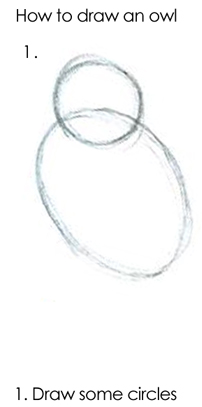
\includegraphics[height=0.8\textheight]{images/owl_1.png}
  \pause
  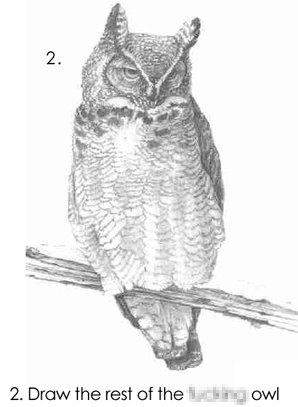
\includegraphics[height=0.8\textheight]{images/owl_2.png}

\end{frame}

\begin{frame}{What's the plan?}
  \large
  \begin{itemize}
    \addtolength{\itemsep}{1ex}
    \item A little bit about \hl{agent-based models} (ABM)
    \item A little bit about the \hl{Poseidon} fisheries ABM
    \item A little bit about the \hl{NetLogo} modelling platform
    \item A whole lot about building \hl{Poseidon in NetLogo}!
  \end{itemize}
\end{frame}

\begin{frame}{Early ABM: Schelling's models of segregation}
  \centering\vskip1em
  
\includegraphics[width=0.4\textwidth]{images/schelling_before.png}\quad
  \visible<2>{%
    
\includegraphics[width=0.4\textwidth]{images/schelling_after.png}
    \vspace{1em}
    Proportion of similar neighbours wanted: 30\%.
  }
\end{frame}

\begin{frame}[t]\frametitle{Examples from the NetLogo model library}
  \begin{columns}[T]\footnotesize
    \begin{column}{0.3\textwidth}
      \centering
      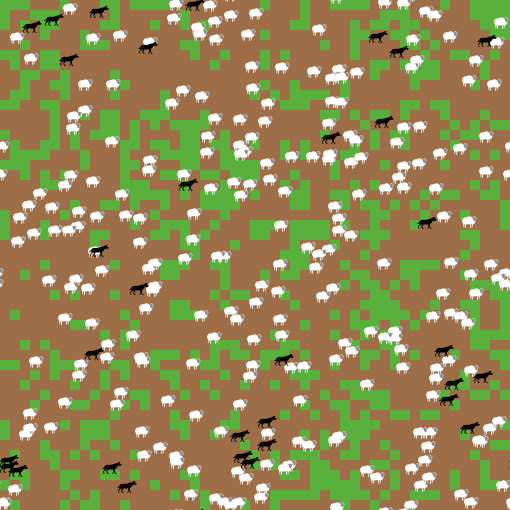
\includegraphics[width=0.7\linewidth]{images/Wolf Sheep Predation.png}\\
      Wolf Sheep Predation
      \vskip 1ex
      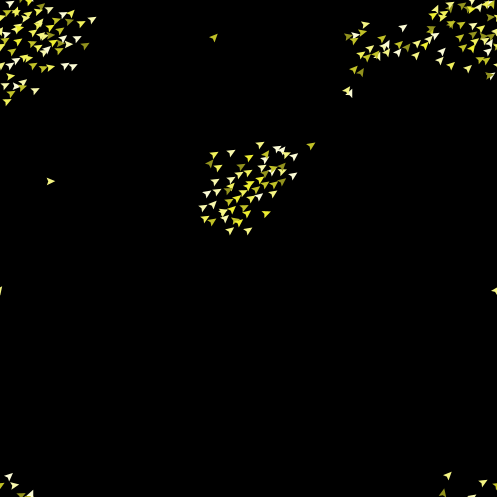
\includegraphics[width=0.7\linewidth]{images/Flocking.png}\\
      Flocking
    \end{column}
    \begin{column}{0.3\textwidth}
      \centering
      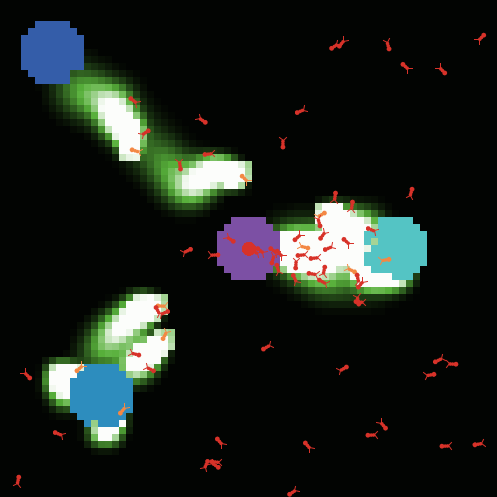
\includegraphics[width=0.7\linewidth]{images/Ants.png}\\
      Ants
      \vskip 1ex
      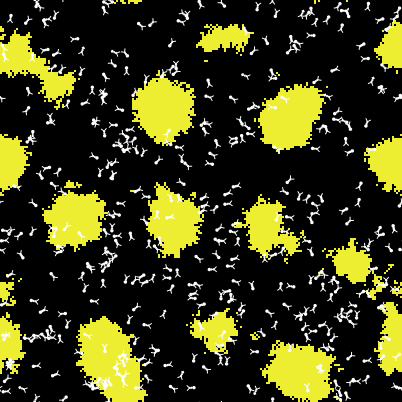
\includegraphics[width=0.7\linewidth]{images/Termites.png}\\      
      Termites
    \end{column}
    \begin{column}{0.3\textwidth}
      \centering
      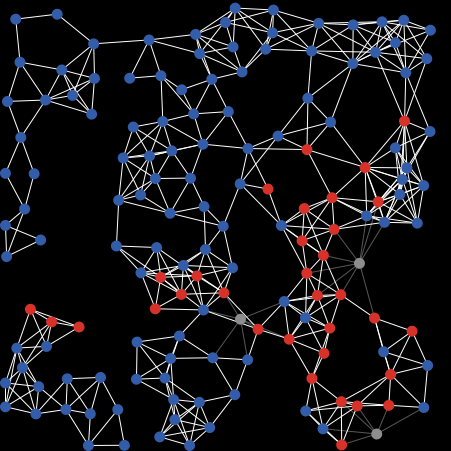
\includegraphics[width=0.7\linewidth]{images/Virus on a Network.png}\\
      Virus on a Network
      \vskip 5ex
      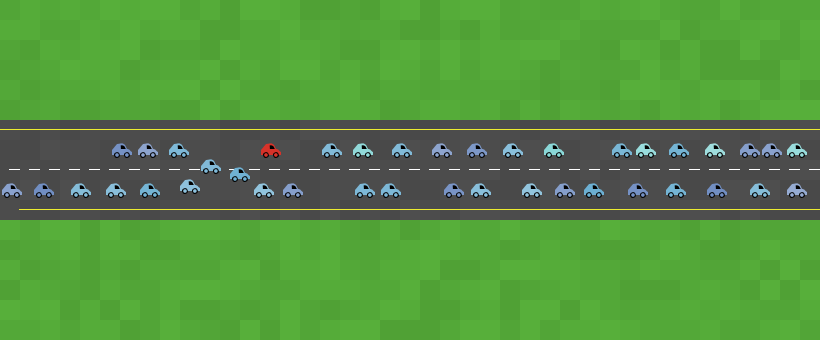
\includegraphics[width=0.7\linewidth]{images/Traffic 2 Lanes.png}\\
      Traffic 2 Lanes
    \end{column}
  \end{columns}
\end{frame}

\begin{frame}{Some typical characteristics of ABM}
  \setbeamersize{description width=10em}
  \small
  \begin{description}
    \item [Heterogeneity:] agents have their own individual properties and can differ from one another.
    \item [Autonomy:] agents makes their own decisions; there is no central control.
    \item [Explicit space:] agents are located in a well-defined environment (e.g., a network or a grid).
    \item [Local interactions:] agents interact with their neighours and their local environment.
    \item [Bounded rationality:] agents are not omnicient and often use behavioural heuristics.
  \end{description}
  \vfill
  \tiny See: Epstein, Joshua M. 2006. Generative Social Science: Studies in Agent-Based Computational Modeling. Princeton University Press.
\end{frame}

\begin{frame}
  \centering
  \vskip 1ex
  
\includegraphics[height=0.8\textheight]{images/mechanism.png}
\end{frame}

\begin{frame}
  \begin{columns}[T]
    \begin{column}{0.35\textwidth}
      \Large\hl{Why model?}\\
      \vskip 1cm
      \tiny Epstein, J. M. 2008. Journal of Artificial Societies and Social Simulation 11(4):12. \url{http://jasss.soc.surrey.ac.uk/11/4/12.html}
    \end{column}
    \begin{column}{0.65\textwidth}
      \scriptsize
      \begin{enumerate}
        \item Explain (very distinct from predict)
        \item Guide data collection
        \item Illuminate core dynamics
        \item Suggest dynamical analogies
        \item Discover new questions
        \item Promote a scientific habit of mind
        \item Bound (bracket) outcomes to plausible ranges
        \item Illuminate core uncertainties.
        \item Offer crisis options in near-real time
        \item Demonstrate tradeoffs / suggest efficiencies
        \item Challenge the robustness of prevailing theory through perturbations
        \item Expose prevailing wisdom as incompatible with available data
        \item Train practitioners
        \item Discipline the policy dialogue
        \item Educate the general public
        \item Reveal the apparently simple (complex) to be complex (simple) 
      \end{enumerate}
    \end{column}    
  \end{columns}
\end{frame}

\begin{frame}{Why model fisheries?}
    
  \begin{itemize}
    \item It's big!
      \begin{itemize}
        \item 96.4 million tonnes of fish caught in 2018
        \item employing 59.51 million people
        \item 17\% of total animal protein consumed globally
      \end{itemize}
    \vfill
    \item It's in trouble!
      \begin{itemize}
        \item 34.2\% of stocks are overfished
      \end{itemize}
  \end{itemize}
  \vfill
  \hl{Why use ABM to do it?}
  \begin{itemize}
    \item They're inherently spatial;
    \item they involve complex interactions,
    \item between smart, adaptive agents.
  \end{itemize}
  \vfill
  \tiny Source: \url{http://www.fao.org/3/ca9231en/CA9231EN.pdf}
\end{frame}

\begin{frame}
  \begin{columns}[T]
    \begin{column}{0.35\textwidth}
      \Large\hl{Poseidon}
      \vskip 1ex
      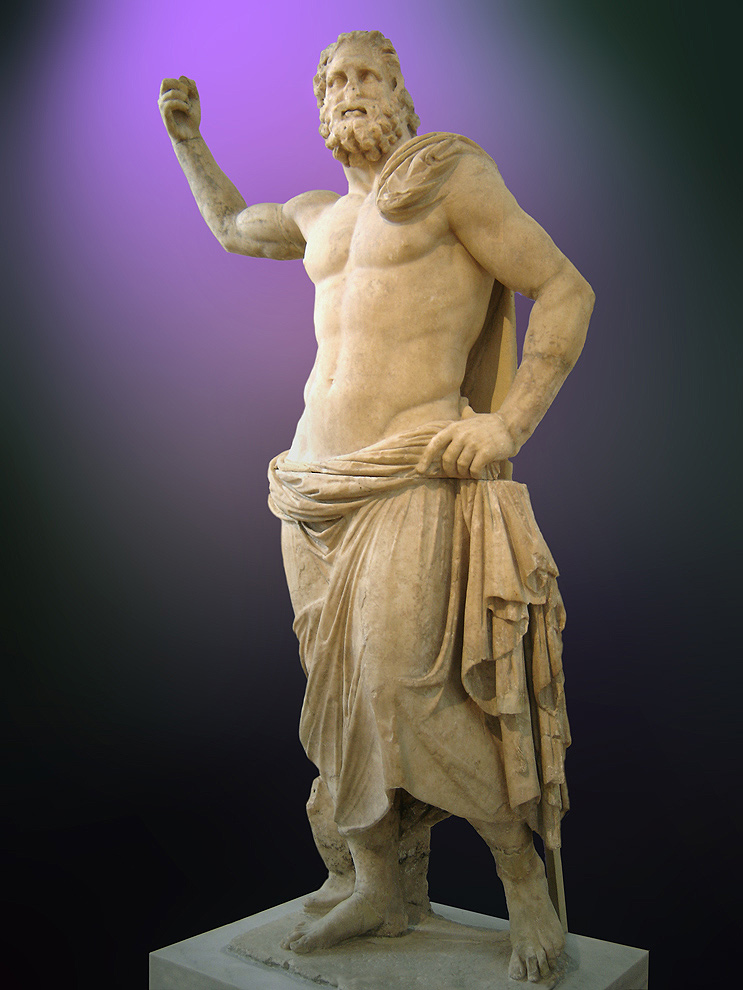
\includegraphics[width=\linewidth]{images/0036MAN_Poseidon}
      \tiny Source: Ricardo André Frantz, \url{https://w.wiki/wzx}
    \end{column}
    \begin{column}{0.65\textwidth}
      \hfill
      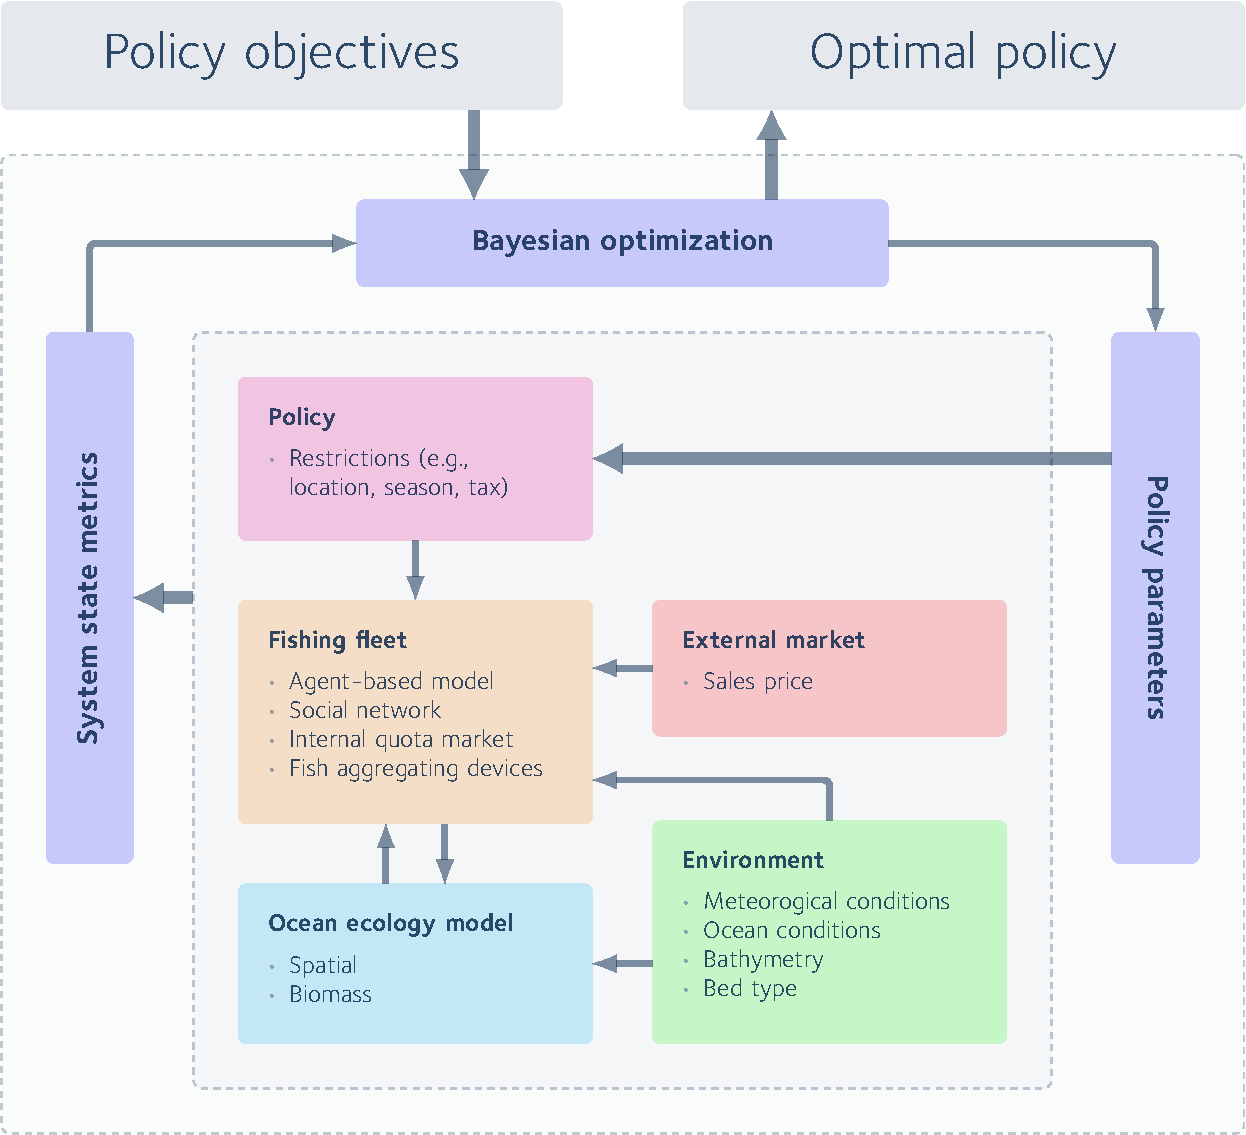
\includegraphics[height=0.95\textheight]{images/poseidon_diagram.pdf}
    \end{column}    
  \end{columns}
\end{frame}

\begin{frame}[t]\frametitle{Poseidon applications}
  \begin{columns}[T]
    \begin{column}{0.575\textwidth}
      \footnotesize
      \begin{itemize}
        \item Conceptual models
        \item US West Coast Groundfish
        \item Indonesian Deep water snapper grouper fishery
        \item Eastern Pacific Tuna Management
      \end{itemize}
      \vskip 1em
      
\includegraphics[width=\linewidth]{images/Design-Partners.png}
    \end{column}
    \begin{column}{0.425\textwidth}
      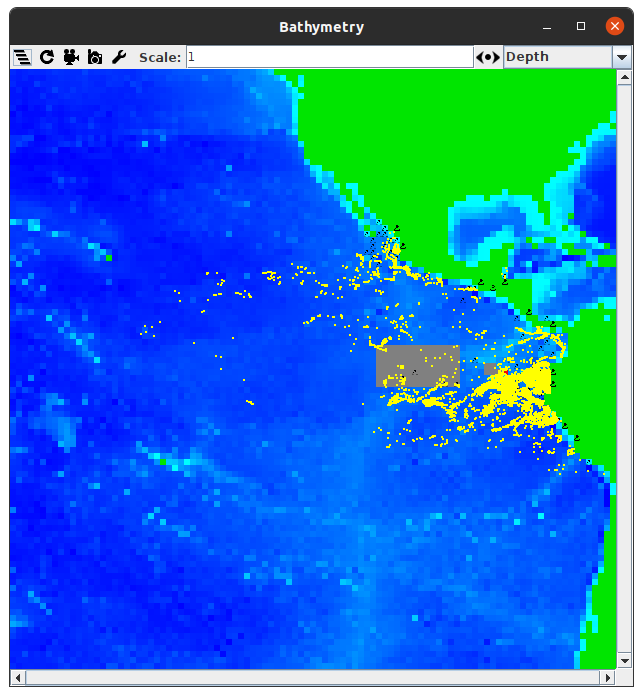
\includegraphics[width=\linewidth]{images/poseidon_screenshot.png}
    \end{column}
  \end{columns}
\end{frame}


\begin{frame}[t]\frametitle{What can we put in a minimal fisheries model?}
  \Large
  \vfill
  \begin{columns}[T]
    \begin{column}{0.4\textwidth}
      \hl{Agents:}
      \begin{itemize}
        \item A port,
        \item fishers,
        \item and fish!
      \end{itemize}
    \end{column}
    \begin{column}{0.6\textwidth}
      \hl{Some policy to test:}
      \begin{itemize}
        \item The size of a marine protected area (MPA)
      \end{itemize}
    \end{column}
  \end{columns}
  \vfill
\end{frame}

\begin{frame}[t]
  \Large Fisher agents in Poseidon use the\\\hl{``Explore, exploit, imitate''}\\behaviour algorithm:
  \vfill
  \begin{tcolorbox}[halign=flush left]
  \begin{itemize}\small
    \item Should I go exploring?
    \begin{itemize}\small
      \item If yes, pick a random spot not too far from my favourite spot (\hl{EXPLORE})
      \item If not, pick a friend and ask: is my favourite spot better than my friend's favourite spot?
      \begin{itemize}\small
        \item If it is, go to my favourite spot (\hl{EXPLOIT})
        \item If it isn't, go to my friend's favourite spot (\hl{IMITATE})
      \end{itemize}
    \end{itemize}
    \item If the spot I went to was better than my favourite spot, it becomes my new favourite!
  \end{itemize}
  \end{tcolorbox}
\end{frame}

\begin{frame}[t]\frametitle{A bit of biology}
  \begin{columns}
    \begin{column}{0.7\textwidth}
      {\small We do not simulate individual fish. We keep track of the total biomass and apply yearly \hl{logistic growth}.}
      $$\frac{dP}{dt}=r P \left(1 - \frac{P}{K}\right)$$
      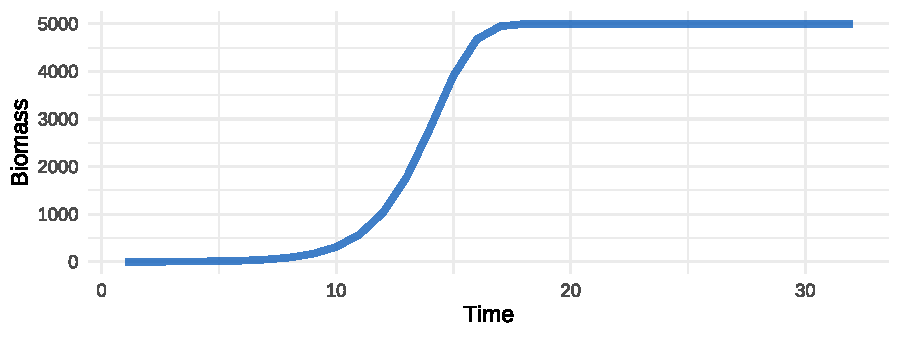
\includegraphics[width=\linewidth]{images/logistic_growth.pdf}
    \end{column}
    \begin{column}{0.3\textwidth}
      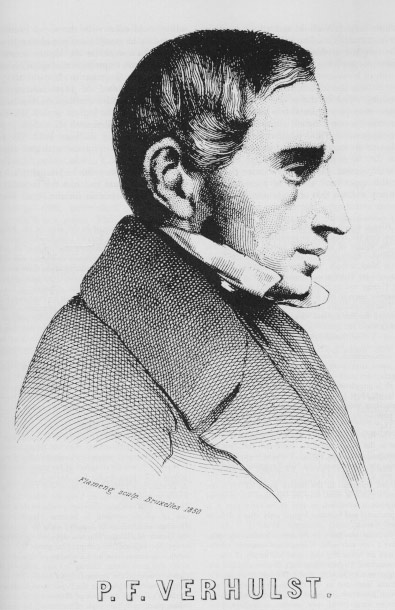
\includegraphics[width=\linewidth]{images/Pierre_Francois_Verhulst.jpg}\\
      \tiny Pierre-François Verhulst (1804--1849).\\Source: \url{https://w.wiki/x2o}.
    \end{column}
  \end{columns}

\end{frame}

\begin{frame}[t]\frametitle{ABM frameworks}
  \footnotesize
  \begin{itemize}
    \item
      \hl{NetLogo} (Logo)\\
      \url{https://ccl.northwestern.edu/netlogo/}
    \item
      \hl{MASON} (Java; MASON is what we use for Poseidon)\\
      \url{https://cs.gmu.edu/~eclab/projects/mason/}\\
    \item
      \hl{MESA} (Python)\\
      \url{https://github.com/projectmesa/mesa/}
    \item
      \hl{Repast} (Groovy or Java)\\
      \url{https://repast.github.io/}      
    \item
      \hl{GAMA} ("GAMA agent modelling language")\\
      \url{https://gama-platform.github.io/}      
    \item
      \hl{HASH} (Python or JavaScript; free but \hl{not} open-source)\\
      \url{https://hash.ai/}
  \end{itemize}
\end{frame}

\begin{frame}{Why NetLogo?}
  \begin{columns}[T]
    \begin{column}{0.5\textwidth}\small
      \begin{itemize}
        \item \emph{Lingua franca} of the ABM community
        \item All-in-one IDE for GUI building / model coding / experiment running
        \item Logo language optimized for ABM
        \item ``Low threshold, high ceiling'' (i.e., more powerful than you think)
      \end{itemize}
    \end{column}
    \begin{column}{0.5\textwidth}
      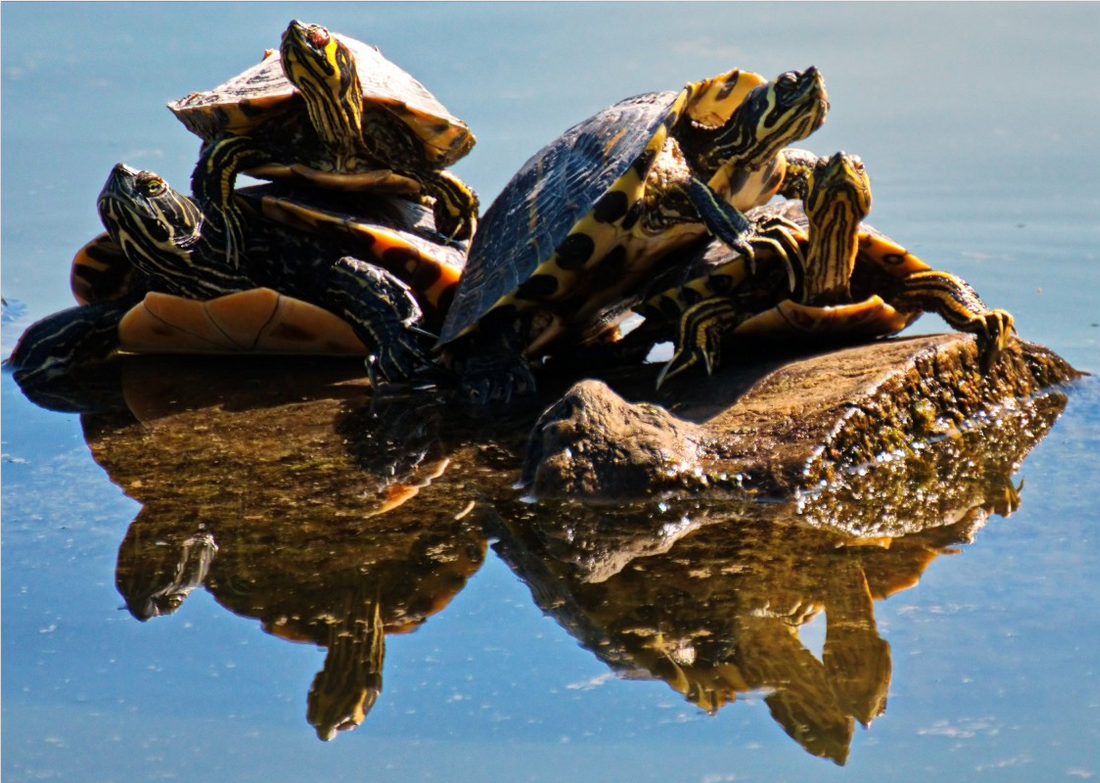
\includegraphics[width=\linewidth]{images/turtles.png}
    \end{column}
  \end{columns}
\end{frame}

\begin{frame}
  \begin{columns}[T]
    \begin{column}{0.6\textwidth}\Large
      \hl{Agents in NetLogo}
      \vskip 1em
      Turtles, patches and links
      \vskip 1em
      
\includegraphics[height=0.5\textheight]{images/turtles_patches_links.png}
    \end{column}
    \begin{column}{0.4\textwidth}
      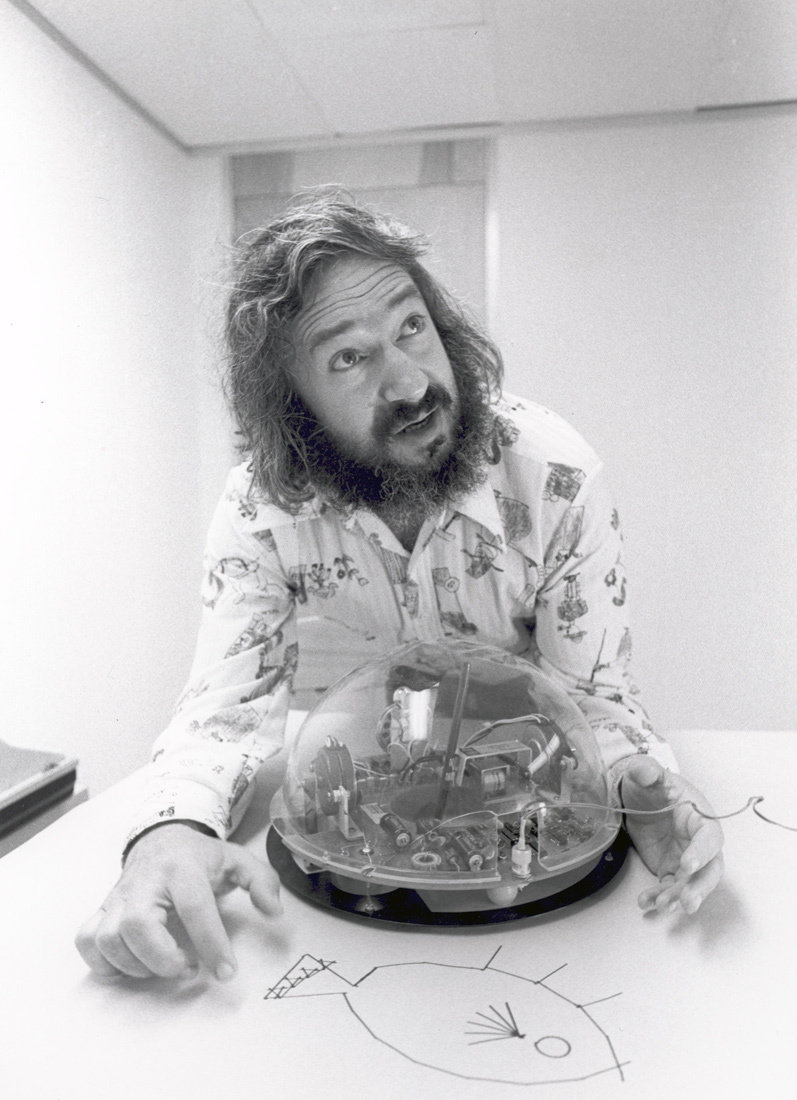
\includegraphics[height=0.8\textheight]{images/papert.jpeg}\\
      \tiny Seymour Papert, 1928--2016\\(Credit: Cynthia Solomon/MIT Media Lab)
    \end{column}    
  \end{columns}
\end{frame}

\begin{frame}[fragile=singleslide]{Basic skeleton of a NetLogo model}
  \begin{columns}
    \begin{column}{0.55\textwidth}
      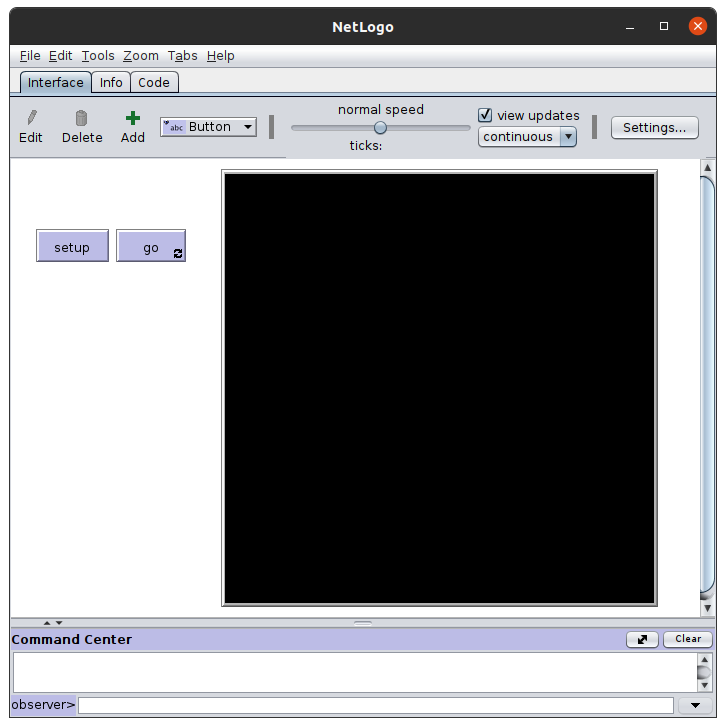
\includegraphics[height=0.8\textheight]{images/skeleton}\\
    \end{column}
    \begin{column}{0.45\textwidth}
      \begin{adjustbox}{max width=\linewidth}
        \begin{nlogo}
 to setup
   clear-all
   reset-ticks
 end

 to go
   tick
 end
        \end{nlogo}
      \end{adjustbox}
    \end{column}
  \end{columns}  
\end{frame}


\begin{frame}[fragile=singleslide]{Creating a port}
  \begin{columns}
    \begin{column}{0.45\textwidth}
    \small
    \begin{minted}[highlightlines={1, 5-9}]{nlogo}
 breed [ ports port ]

 to setup
   clear-all
   create-ports 1 [
     set xcor max-pxcor
     set color lime
     set shape "square"
   ]
   reset-ticks
 end
        \end{minted}
    \end{column}
    \begin{column}{0.55\textwidth}
      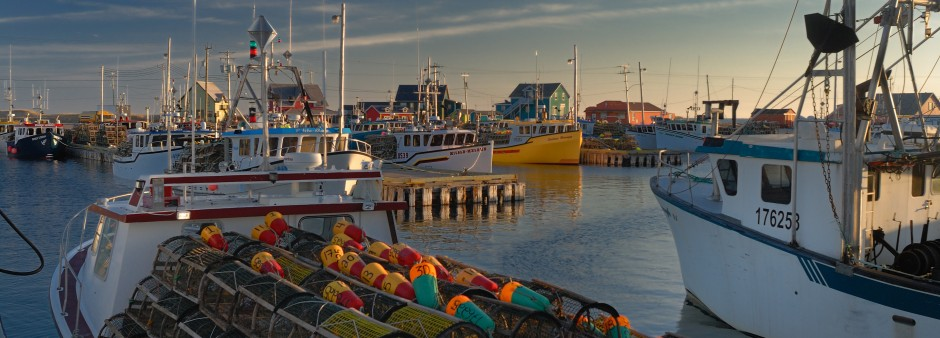
\includegraphics[width=\textwidth]{images/port.jpg}\\
      \tiny Source: \url{https://www.tourismeilesdelamadeleine.com/fr/decouvrir-les-iles/les-iles/ile-de-grande-entree}
    \end{column}
  \end{columns}
\end{frame}

\begin{frame}[fragile=singleslide]{Adding some fish biomass}\small
  \begin{minted}[highlightlines={2, 11}]{nlogo}
 breed [ ports port ]
 patches-own [ biomass ]
 
 to setup
   clear-all
   create-ports 1 [
     set xcor max-pxcor
     set color lime
     set shape "square"
   ]
   ask patches [ set biomass carrying-capacity ]
   reset-ticks
 end
  \end{minted}  
\end{frame}

\begin{frame}{Adding a \texttt{carrying-capacity} slider}
  \centering\vfill
  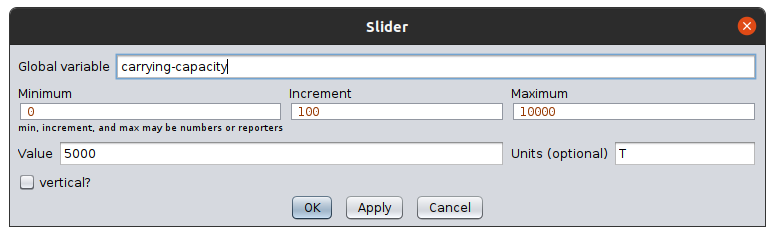
\includegraphics[width=\linewidth]{images/carrying_capacity_slider.png}
  \vfill
\end{frame}


\begin{frame}[fragile=singleslide]\frametitle{Recoloring patches}
  \centering
  \begin{adjustbox}{max width=\linewidth}
    \begin{nlogo}
to recolor-patches
  ask patches [
    set pcolor scale-color blue (biomass / 2) carrying-capacity 0
  ]
end
    \end{nlogo}
  \end{adjustbox}
  \vfill
  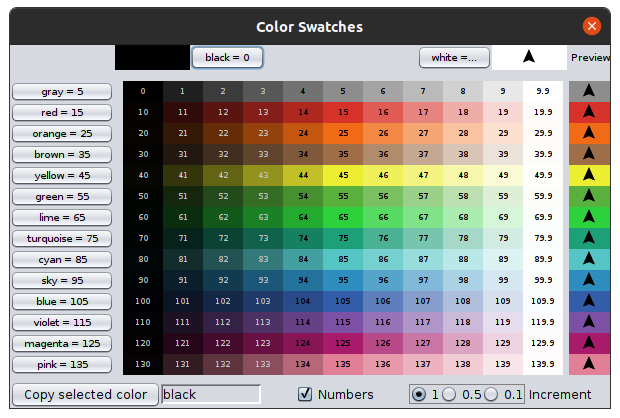
\includegraphics[width=0.7\textheight]{images/swatches.png}
\end{frame}

\begin{frame}[fragile=singleslide]{Calling \texttt{recolor-patches} from \texttt{setup}}\small
  \begin{minted}[highlightlines={9}]{nlogo}
to setup
  clear-all
  create-ports 1 [
    set xcor max-pxcor
    set color lime
    set shape "square"
  ]
  ask patches [ set biomass carrying-capacity ]
  recolor-patches
  reset-ticks
end
  \end{minted}  
\end{frame}

\begin{frame}[fragile=singleslide]{Creating some fishers}\scriptsize
  \begin{minted}[highlightlines={2,14-17}]{nlogo}
 breed [ ports port ]
 breed [ fishers fisher ]
 patches-own [ biomass ]
 
 to setup
   clear-all
   create-ports 1 [
     set xcor max-pxcor
     set color lime
     set shape "square"
   ]
   ask patches [ set biomass carrying-capacity ]
   recolor-patches  
   create-fishers number-of-fishers [
     set color yellow
     move-to one-of ports
   ]
   reset-ticks
 end
  \end{minted}  
\end{frame}


\begin{frame}{Adding a \texttt{number-of-fishers} slider}
  \centering\vfill
  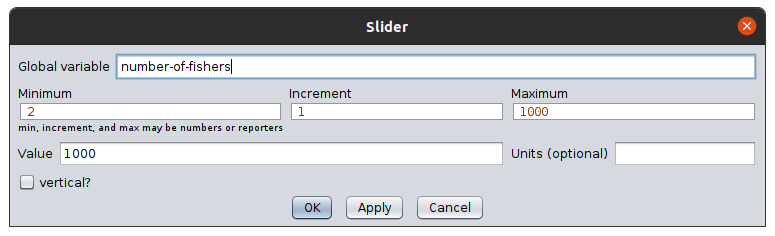
\includegraphics[width=\linewidth]{images/numer_of_fishers_slider.png}
  \vfill
\end{frame}

\begin{frame}[fragile=singleslide]{Creating a marine protected area}
  \begin{adjustbox}{max width=\linewidth}
    \begin{nlogo}
globals [ fishable-patches ] ; put this at the very top of the code tab
breed [ xs x ] ; put this before the other breed declarations

to setup-mpa
  set-default-shape xs "x"
  let mpa patches with [ abs pxcor < mpa-border and abs pycor < mpa-border ]
  ask mpa [ sprout-xs 1 [ set color cyan ] ]
  set fishable-patches patches with [ not member? self mpa ]
end
    \end{nlogo}
  \end{adjustbox}
  \vfill
  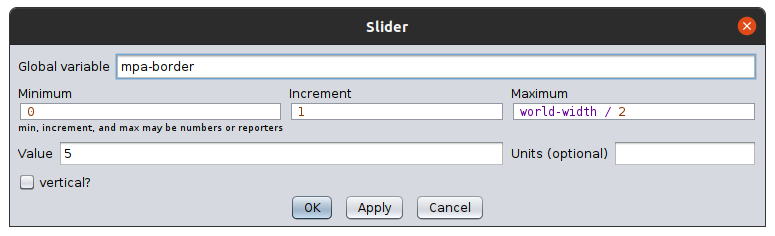
\includegraphics[height=0.35\textheight]{images/map_border_slider.png}
\end{frame}

\begin{frame}[fragile=singleslide]{Calling \texttt{setup-mpa} from the \texttt{setup} procedure}\scriptsize
  \begin{minted}[highlightlines={14}]{nlogo}
 breed [ ports port ]
 breed [ fishers fisher ]
 patches-own [ biomass ]
 
 to setup
   clear-all
   create-ports 1 [
     set xcor max-pxcor
     set color lime
     set shape "square"
   ]
   ask patches [ set biomass carrying-capacity ]
   recolor-patches
   setup-mpa
   create-fishers number-of-fishers [
     set color yellow
     move-to one-of ports
   ]
   reset-ticks
 end
  \end{minted}  
\end{frame}

\begin{frame}
  \centering\vfill\Large
  \hl{Now, a bit of house keeping\ldots}
  \vfill
\end{frame}

\begin{frame}\frametitle{Adjusting the model settings}
  \begin{columns}
    \begin{column}{0.35\textwidth}
      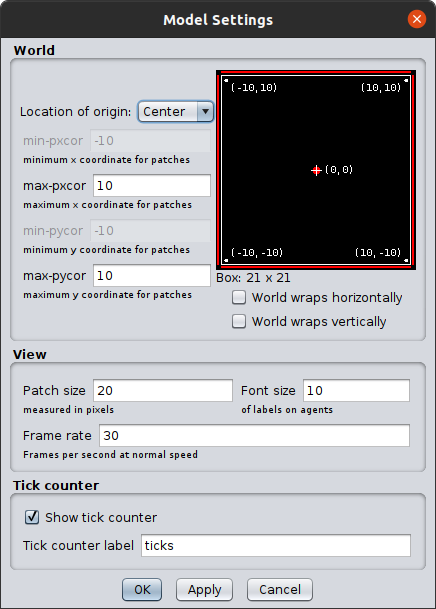
\includegraphics[width=\textwidth]{images/model_settings.png}
    \end{column}
    \begin{column}{0.65\textwidth}
      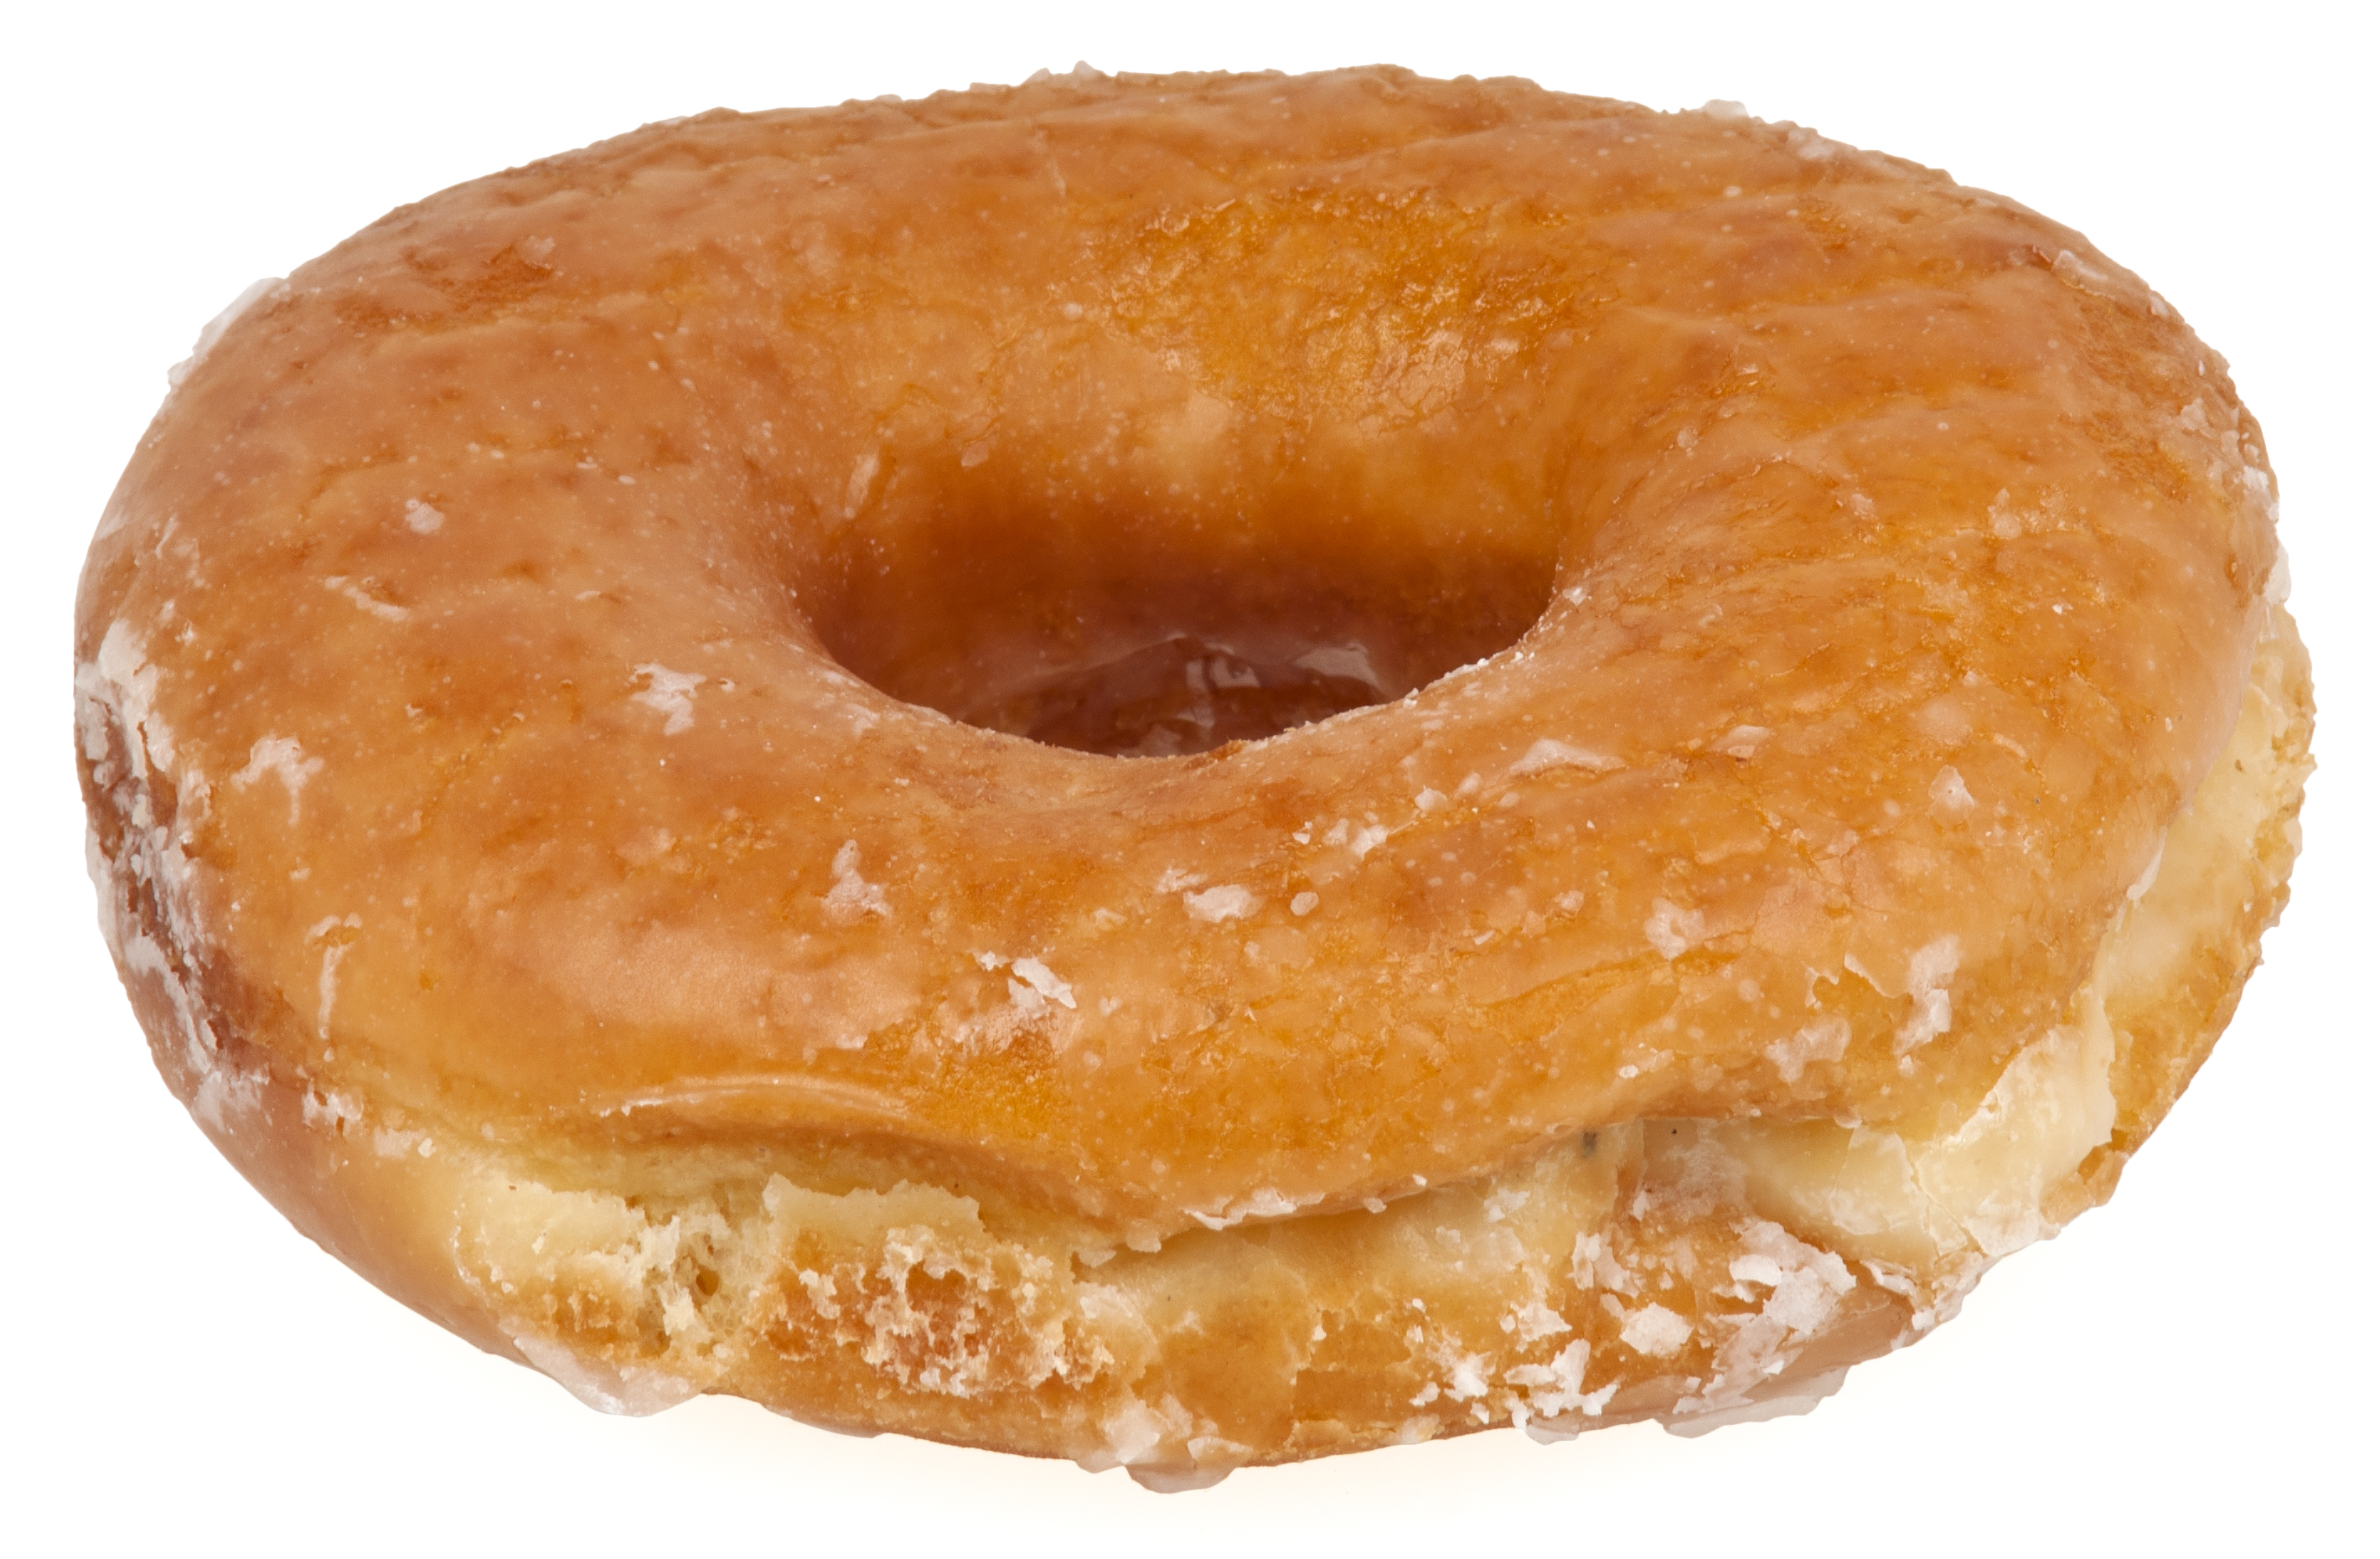
\includegraphics[width=\textwidth]{images/Glazed-Donut.jpg}
    \end{column}    
  \end{columns}
\end{frame}

\begin{frame}[fragile=singleslide]{Creating sliders and fisher variables}
  \begin{columns}[T]
    \begin{column}{0.3\textwidth}
      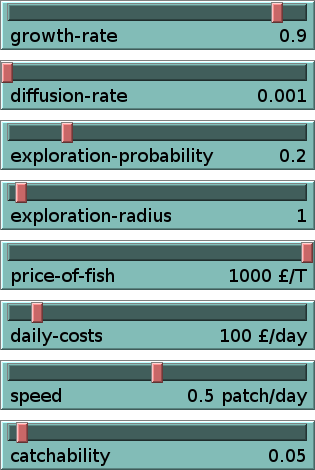
\includegraphics[width=\linewidth]{images/sliders.png}      
    \end{column}
    \begin{column}{0.7\textwidth}\small
      \begin{nlogo}
  ; this goes at the top, as always
  fishers-own [
    favourite-destination
    profits-at-favourite-destination
    current-destination
    trip-destination
    trip-costs
    bank-balance
    biomass-in-hold
  ]
      \end{nlogo}
    \end{column}
  \end{columns}
\end{frame}

\begin{frame}[fragile=singleslide]{Let's \texttt{go}!}
  \begin{adjustbox}{max width=\linewidth}\small
  \begin{minted}[]{nlogo}
to go
  ask fishers [
    set trip-costs trip-costs + daily-costs
    ifelse patch-here = current-destination [
      ifelse any? ports-here [ dock ] [ fish ]
    ] [
      face current-destination
      forward speed
    ]
  ]
  tick
end
    \end{minted}
  \end{adjustbox}
\end{frame}

\begin{frame}[fragile=singleslide]\frametitle{Fishing!}
  \begin{adjustbox}{max width=\linewidth}
    \begin{nlogo}
to fish ; fisher procedure
  let biomass-caught biomass * catchability
  set biomass biomass - biomass-caught
  set biomass-in-hold biomass-in-hold + biomass-caught
  set current-destination [ patch-here ] of one-of ports
  set pcolor red
end    
    \end{nlogo}
  \end{adjustbox}
\end{frame}


\begin{frame}[fragile=singleslide]{Docking at the port}
  \begin{adjustbox}{max height=0.8\textheight}
    \begin{nlogo}
to dock ; fisher procedure
  let revenues biomass-in-hold * price-of-fish
  set biomass-in-hold 0
  let profits revenues - trip-costs
  set trip-costs 0
  set bank-balance bank-balance + profits

  ifelse trip-destination = favourite-destination [
    set profits-at-favourite-destination profits
  ] [
    if profits > profits-at-favourite-destination [
      set favourite-destination trip-destination
      set profits-at-favourite-destination profits
    ]
  ]
  pick-destination
end
    \end{nlogo}
  \end{adjustbox}
\end{frame}


\begin{frame}[fragile=singleslide]{Exploring, exploiting, imitating}
  \begin{adjustbox}{max width=\linewidth}
    \begin{nlogo}
to pick-destination ; fisher procedure
  ifelse random-float 1 < exploration-probability [
    ; explore:
    let r random-poisson exploration-radius
    set trip-destination [ one-of fishable-patches in-radius r ] of favourite-destination
  ] [
    let other-fisher one-of other fishers
    let other-profits [ profits-at-favourite-destination ] of other-fisher
    ifelse profits-at-favourite-destination >= other-profits [
      ; exploit:
      set trip-destination favourite-destination
    ] [
      ; imitate:
      set trip-destination [ favourite-destination ] of other-fisher
    ]
  ]
  set current-destination trip-destination
end
    \end{nlogo}
  \end{adjustbox}
\end{frame}

\begin{frame}[fragile=singleslide]{Calling \texttt{pick-destination} from \texttt{setup}}
  \begin{adjustbox}{max height=0.75\textheight}
  \begin{minted}[highlightlines={15}]{nlogo}
to setup
  clear-all
  create-ports 1 [
    set xcor max-pxcor
    set color lime
    set shape "square"
  ]
  ask patches [ set biomass carrying-capacity ]
  setup-mpa
  recolor-patches
  create-fishers number-of-fishers [
    set color yellow
    move-to one-of ports
    set favourite-destination patch-here
    pick-destination
  ]
  reset-ticks
end
    \end{minted}
  \end{adjustbox}
\end{frame}


\begin{frame}[fragile=singleslide]{Updating the biology}
  \vfill
  $$\frac{dP}{dt}=r P \left(1 - \frac{P}{K}\right)$$
  \vfill
  \begin{adjustbox}{max width=\linewidth}
    \begin{nlogo}
to update-biology
  diffuse biomass diffusion-rate
  recolor-patches
  if ticks mod 365 = 0 [
    ask patches [
      set biomass biomass + (
        growth-rate * biomass * (1 - (biomass / carrying-capacity))
      )
    ]
  ]
end
    \end{nlogo}
  \end{adjustbox}
\end{frame}

\begin{frame}[fragile=singleslide]{Calling \texttt{update-biology} from \texttt{go}}
  \begin{adjustbox}{max width=\linewidth}\small
  \begin{minted}[highlightlines={11}]{nlogo}
to go
  ask fishers [
    set trip-costs trip-costs + daily-costs
    ifelse patch-here = current-destination [
      ifelse any? ports-here [ dock ] [ fish ]
    ] [
      face current-destination
      forward speed
    ]
  ]
  update-biology
  tick
end
    \end{minted}
  \end{adjustbox}
\end{frame}


\begin{frame}{Adding a couple of plots}
  \vfill
  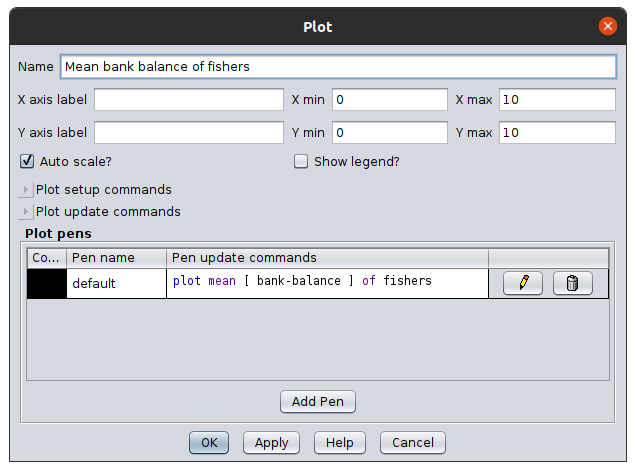
\includegraphics[width=0.49\linewidth]{images/plot_balance.png}\hfill
  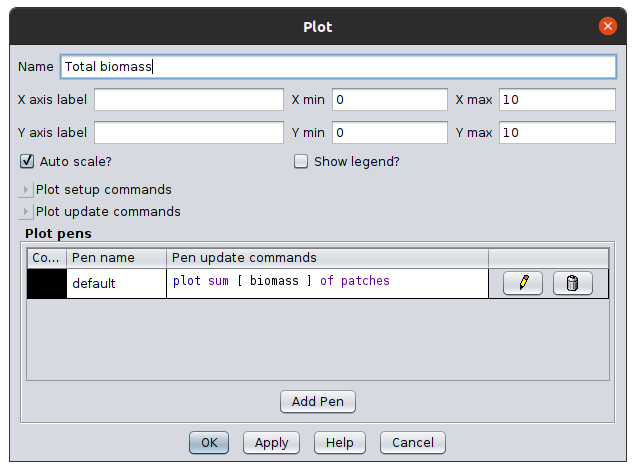
\includegraphics[width=0.49\linewidth]{images/plot_biomass.png}
  \vfill
\end{frame}

\begin{frame}[fragile=singleslide]{}
  \begin{columns}[T]
    \begin{column}{0.5\textwidth}
      {\Large Running an automated experiment through \hl{BehaviorSpace}}
      \vfill
      \small
      \begin{verbatim}
["price-of-fish" 1000]
["mpa-border" [0 1 9]]
["carrying-capacity" 5000]
["exploration-probability" 0.2]
["catchability" 0.05]
["speed" 0.5]
["number-of-fishers" 1000]
["daily-costs" 100]
["diffusion-rate" 0.001]
["exploration-radius" 1]
["growth-rate" 0.9]
      \end{verbatim}

    \end{column}
    \begin{column}{0.5\textwidth}
      \hfill
      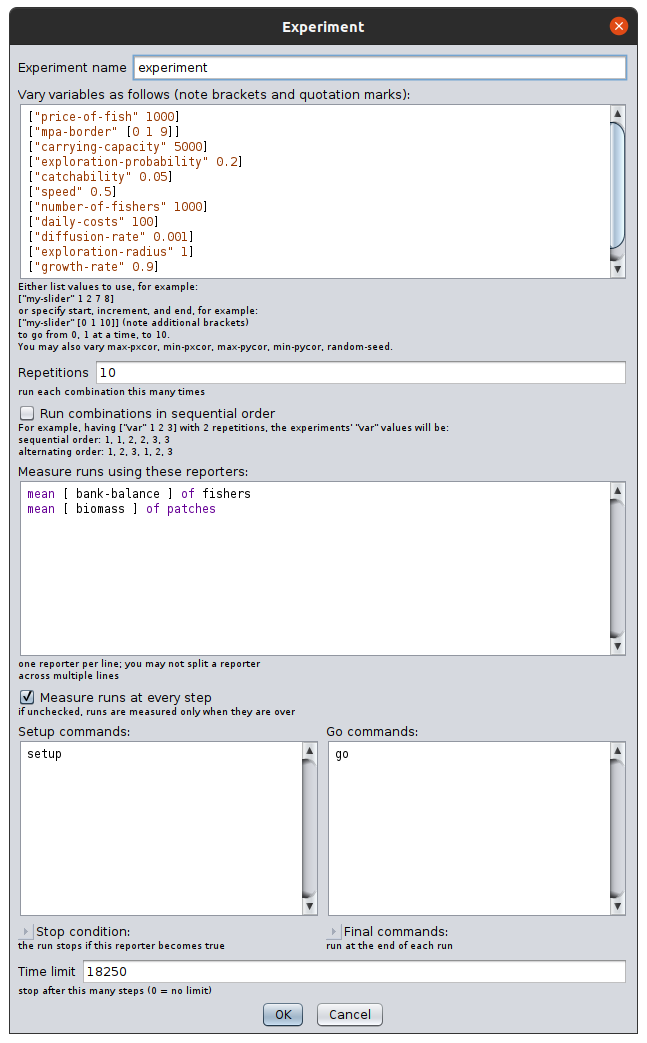
\includegraphics[height=0.95\textheight]{images/behavior_space.png}
    \end{column}    
  \end{columns}
\end{frame}

\begin{frame}{}
  \makebox[\textwidth]{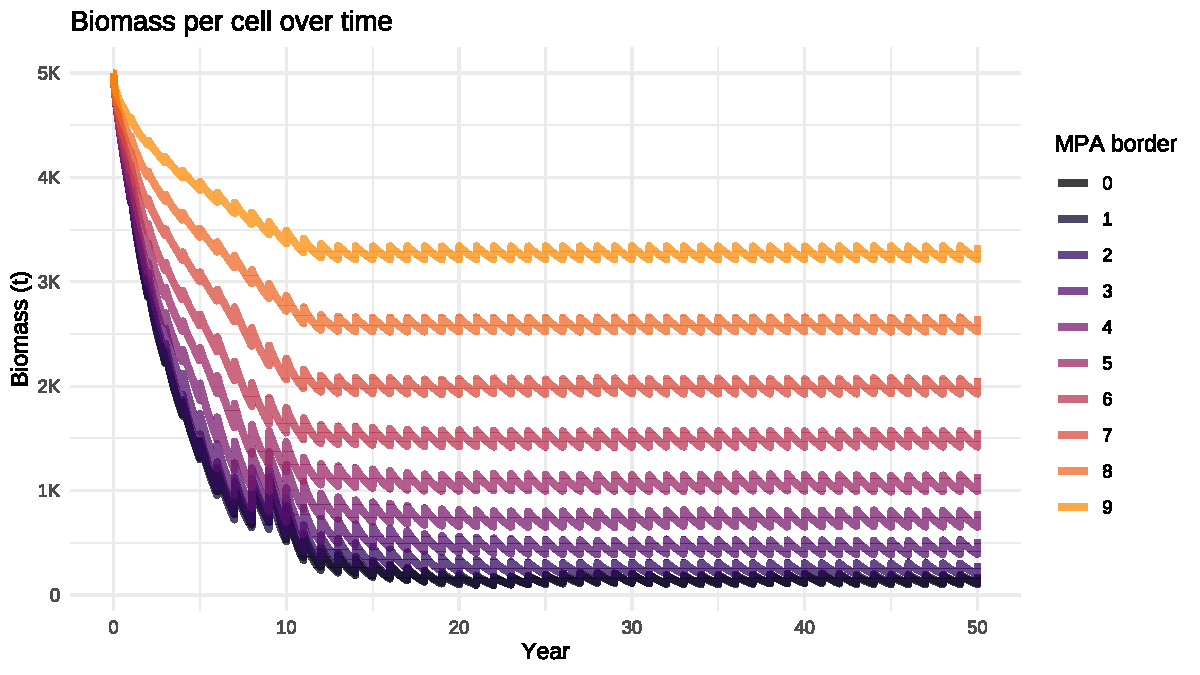
\includegraphics[width=\paperwidth]{images/biomass}}
\end{frame}

\begin{frame}{}
  \makebox[\textwidth]{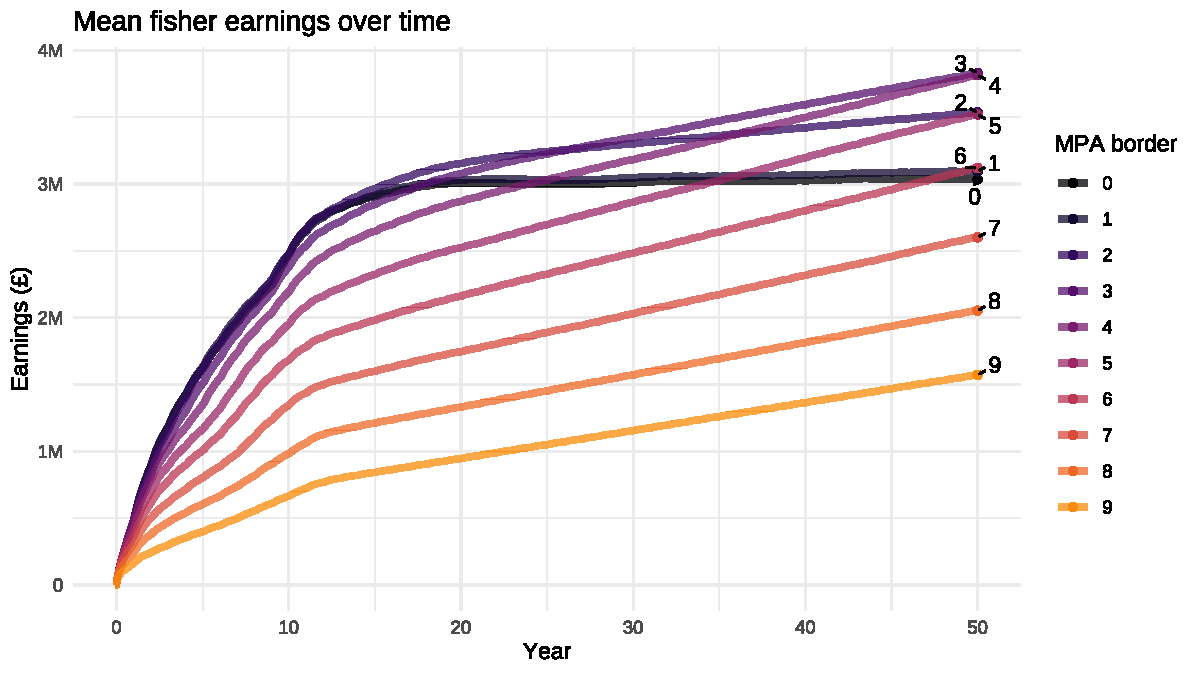
\includegraphics[width=\paperwidth]{images/earnings}}
\end{frame}

\begin{frame}{}
  \makebox[\textwidth]{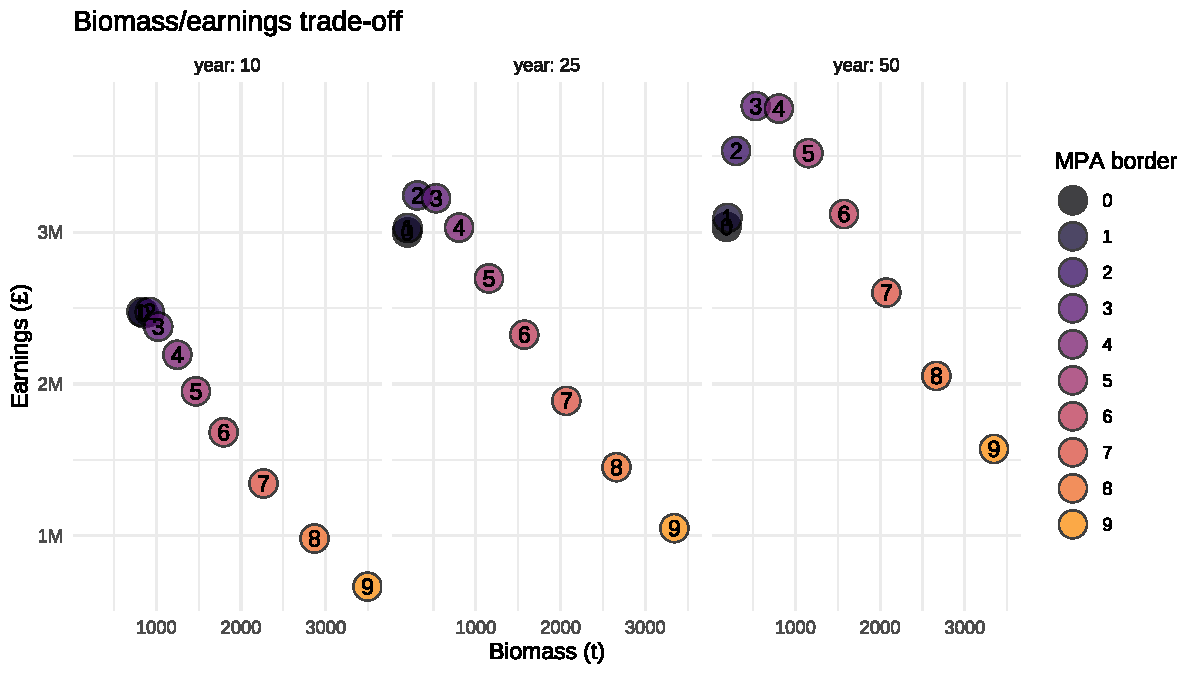
\includegraphics[width=\paperwidth]{images/tradeoff}}
\end{frame}

\begin{frame}{``Homework''}
  \vfill
  \hl{How robust are our results?}
  \begin{itemize}
    \item Which parameters are they sensitive to?
    \item What is the range for which they hold?
  \end{itemize}
  \vfill
  \hl{Can you add exit/entry into the fishery?}
  \begin{itemize}
    \item Hint: agents can \texttt{die} or \texttt{hatch} new agents.
    \item How does that affect the fishery's sustainability?
  \end{itemize}
  \vfill
\end{frame}


\begin{frame}[t]\frametitle{Readings about ABM}\scriptsize

    \vfill    
    \hl{Classics}
    \begin{itemize}
      \item Schelling, Thomas C. 1978. Micromotives and Macrobehavior. Norton.
      \item Resnick, Mitchel. 1997. Turtles, Termites, and Traffic Jams: Explorations in Massively Parallel Microworlds. MIT Press.
      \item Epstein, Joshua M., and Robert Axtell. 1996. Growing Artificial Societies: Social Science from the Bottom Up. Brookings Institution Press.
    \end{itemize}

    \vfill    
    \hl{Textbooks}
    \begin{itemize}
      \item Railsback, Steven F., and Volker Grimm. 2012. Agent-Based and Individual-Based Modeling: A Practical Introduction. Princeton University Press.
      \item Wilensky, Uri, and William Rand. 2015. An Introduction to Agent-Based Modeling: Modeling Natural, Social and Engineered Complex Systems with NetLogo. Cambridge, MA: MIT Press.
    \end{itemize}

    \vfill    
    \hl{Current research}
    \begin{itemize}
      \item Journal of Artifical Societies and Social Simulation\\\url{http://jasss.soc.surrey.ac.uk}
    \end{itemize}


    \vfill    
    \hl{Other resources}
    \begin{itemize}
      \item \url{https://ccl.northwestern.edu/netlogo/resources.shtml}
      \item \url{https://www.jiscmail.ac.uk/cgi-bin/webadmin?A0=simsoc}
    \end{itemize}

\end{frame}


\end{document}
